\chapter{Konzept}
\section{Allgemein}
\subsection{Zweck}

\subsection{Ausgangslage}
Als Rich Client Framework wird Eclipse 3.x\footnote{die aktuelle Version ist 3.7 (stand: 31.8.2011)} genommen. Siehe Abschnitt \titleref{selection_rcp_fw}. In der Folge werden die für die Eclipse Plattform gebräuchlichen Begrifflichkeiten verwendet. 

\section{Generelle Informationen}
\subsection{Speicherung des Zustands einer View}\label{memento}
Die Speicherung des Zustands einer View kann implementiert werden, indem die Methode \textit{saveState(memento:IMemento)} überschrieben wird. \textit{IMemento} ist eine Eclipse-Klasse und gleichzeitig die Abstraktion eines Mementos. Mementos dienen zur Serialisierung von Objekten und haben den Vorteil, dass sie nicht an eine Version der Klasse gebunden sind. Das Eclipse-Framework persistiert die Zustände von Views mittels eines XMLMemento entsprechend im XML-Format ab. Die Deserialisierung erreicht man mit dem Überschreiben der Methode \textit{init(site:IViewSite, memento:IMemento)}.

\section{Architektur}
\subsection{Problemstellung}\label{konzept_uebersicht}
Aufgrund der Anforderung QRQ-S-01 (Erweiterbarkeit) muss die Analyse-Software auch hinsichtlich anderer Log-Formate erweiterbar sein. Die Applikation wird also nicht zwingendermassen mit der Erweiterung für JRockit Log Dateien verwendet. Es könnte zu einem späteren Zeitpunkt sein, dass man damit Garbage Collection Logs der HotSpot Virtual Machine auswertet. Dies hat hinsichtlich Architektur einige Konsequenzen:
\begin{itemize}
	\item Die Applikation soll in zwei Komponenten aufgeteilt werden:
		\begin{itemize}
			\item Basissoftware
			\item Erweiterung JRockit
		\end{itemize}
		Die Basissoftware kann unabhängig von den Erweiterungen installiert werden, für die Auswertung einer Log-Datei ist allerdings die entsprechende Erweiterung zu installieren. Eine Erweiterung kann ohne Basissoftware nicht gebraucht werden.
	\item Die Architektur der Applikation muss es zulassen, dass zu einem späteren Zeitpunkt andere Log-Formate als zusätzliche Erweiterungen hinzugefügt werden.
	\item Die Basissoftware stellt Extension-Points\footnote{Ein Extension-Point ist ein Mechanismus der von Eclipse zur Verfügung gestellt wird, damit eine Komponente (Plugin) sich bei einer anderen registrieren kann.} bereit, über welche sich die Erweiterungen  registrieren.
\end{itemize}

\subsection{Übersicht}
Die im Abschnitt \titleref{konzept_uebersicht} beschriebenen Konsequenzen führen dazu, dass die Applikation - obwohl es momentan erst die Erweiterung für die JRockit Garbage Collection Logs gibt - in zwei verschiedene Features aufgeteilt wird. Die beschriebenen Anforderungen können grob folgendermassen zugewiesen werden:
\begin{itemize}
	\item Basissoftware (Core Feature)
		\begin{itemize}
			\item Update der Software
			\item Garbage Collection Log importieren
			\item Garbage Collection Log einlesen
			\item Profil erstellen, speichern, exportieren, importieren
			\item Hilfesystem
		\end{itemize}
	\item JRockit Extension (JRockit Extension Feature)
		\begin{itemize}
			\item Garbage Collection Log parsen
			\item Standardauswertung: Heap, Dauer Garbage Collection
			\item Benutzerdefinierte Auswertung (Administration der Charts)
		\end{itemize}
\end{itemize}

\subsection{Projektstruktur}\label{projektstruktur}
Wie im Abschnitt \titleref{installation} erläutert, besteht die Software aus zwei getrennten Features. Das Core-Feature ist die Basis und verantwortlich für den gesamten Import-Prozess (Import-Wizard, Leseprozess der Log-Datei, Anzeige der Menus, Profil-Verwaltung, etc.). Die JRockit Extension ist eine für die Garbage Collection Logs der JRockit geschriebene Erweiterung. Sie ist für das Parsing der Log-Dateien, die Aufbereitung der Daten und die Anzeige der Charts zuständig. Beinhaltet aber keine Core-Funktionalität.
 \begin{figure}[H]
  	\centering
    	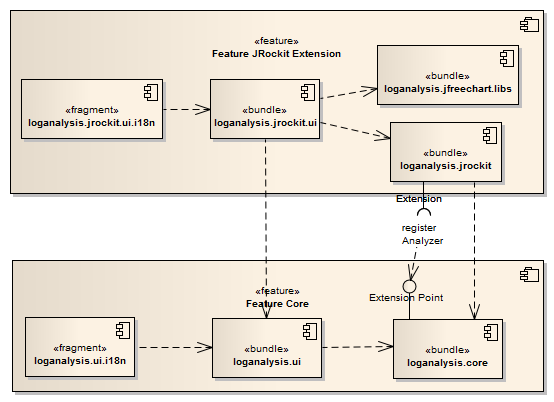
\includegraphics[width=14cm]{images/architektur_komponenten_uebersicht}
        	\caption{Architektur: Komponentendiagramm}
\end{figure}

Das Core Feature besteht aus dem Modul User Interface (``loganalysis.core.ui'') und einem von JFace und SWT\footnote{JFace und SWT wird in Eclipse als Library für den Presentation Layer verwendet} unabhängigen Teil (``loganalysis.core''). Öffnet der Benutzer eine Garbage Collection Log Datei, wird diese durch das Core Feature eingelesen und an alle verfügbaren Extensions weitergeleitet. Die erste Extension welche den Inhalt der Datei versteht, öffnet seine dafür vorgesehenen Reports und Charts. Jede Extension hat ein basierend auf dem Log-Format eigenes Domänen-Modell.

\subsubsection{Weitere Projekte}
Einige Plugins wurden im vorherigen Abschnitt nicht erwähnt:
\begin{itemize}
	\item Test-Projekte\footnote{Der Test-Code befindet sich in eigenen Projekten. Siehe Abschnit \ref{testing} \titleref{testing}}.
		\begin{itemize}
			\item core.test
			\item core.ui.test
			\item jrockit.test
			\item jrockit.ui.test
		\end{itemize}
	\item  Features\footnote{Feature-Projekte definieren im Eclipse-Umfeld ein in sich lauffähiges Software-Packet. Via einen Xml-Deskriptor werden die abhängigen Plugin-Projekte definiert und in das Feature gepackt.}
		\begin{itemize}
			\item loganalysis.feature
			\item loganalysis.jrockit.feature
		\end{itemize}
	\item  Thirdparty Bibliotheken\footnote{Thirdparty Bibliotheken werden ebenfalls in ein Plugin gepackt, da innerhalb der Eclipse-Runntime nur Plugins installiert werden können. Die ``Plugin-Hülle'' definiert die exportierten und importierten Packete und die Abhängigkeiten.}
		\begin{itemize}
			\item  loganalysis.jfreechart.libs (JFreeChart Library)
		\end{itemize}
	\item  Targetplattform\footnote{Die Targetplattform ist eine Konfiguration welche definiert, gegen welche Plattform die Anwendung entwickelt wird.}
		\begin{itemize}
			\item  loganalysis.targetplatform (beinhaltet die Target-Plattform)
		\end{itemize}
	\item  Update-Seite\footnote{Die Konfiguration innerhalb eines Projekts zur Erstellung einer Update-Seite definiert die auf der Seite publizierten Features.}
		\begin{itemize}
			\item loganalysis.updatesite (definiert und generiert die Update-Seite)
		\end{itemize}
\end{itemize}

\subsection{Ablauf Garbage Collection Analyse}
Als Abstraktion für eine Log-Datei wird die Klasse IFileDescriptor verwendet. Beim öffnen einer Analyse wird via den Context die Extension gesucht\footnote{Extensions registrieren sich via das plugins.xml an einem Extension-Point. }, welche den Inhalt\footnote{Der Inhalt der Datei wird lazy via die Methode getContent und einem ContentReader geladen.} der Datei versteht. Sobald die entsprechende Extension gefunden wurde, wird der Inhalt geparst und das Domänenmodell instanziert.
Danach wird der Analyse-Editor mit dem entsprechenden Modellobjekt geöffnet. Der Editor ist ebenfalls sehr proprietär für jedes Log-Format und befindet sich in der jeweiligen Erweiterung (Beispiel JRockitAnalysisEditor). 
 \begin{figure}[H]
  	\centering
    	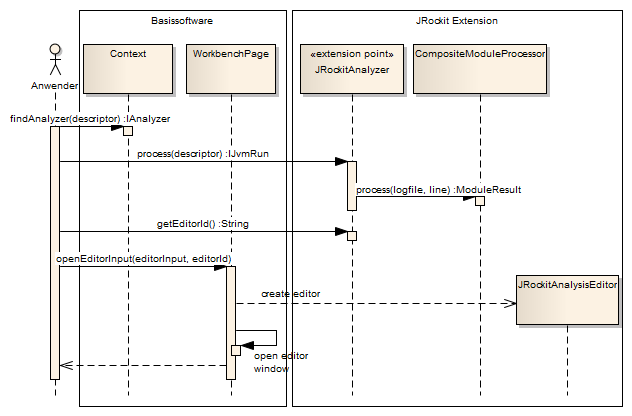
\includegraphics[width=16.5cm]{images/core_sequence_analysis}
	\caption{Sequenz-Diagramm Öffnen der Analyse}
\end{figure}
\section{Basissoftware}
\subsection{Installation}
Für die Installation der Software wird eine Eclipse Update-Seite erstellt. Die Features und damit die Analysesoftware können unter Angabe dieser Seite installiert werden. Die Update-Seite wird wird folgende Softwarepackete beinhalten:
\begin{itemize}
\item \textbf{Basissoftware:} Umfasst alle Plugins , die für die Basissoftware notwendig sind. Siehe Abschnitt \titleref{projektstruktur}.
\item \textbf{JRockit Erweiterung: }Umfasst alle Plugins zur JRockit Erweiterung und hat zugleich die \textbf{Abhängigkeit auf das Basissoftware-Feature}.
\end{itemize}

\subsection{Update}
Der Update eines Features auf der Update-Seite ist erkennbar durch eine Änderung der Major respektive Minor Version oder aber durch Änderung des an die Feature-Datei angehängten Zeitstempels\footnote{Mittels der Versionnummer x.x.qualifier erreicht man, dass der Zeitstempel ans Dateiende gehängt wird.}.

\subsection{Datei importieren}
Der Import einer Log-Datei findet über einen Eclipse-Import-Wizard statt. Der Ablauf zum Import einer oder mehrerer Dateien ist folgendermassen:
\begin{enumerate}
	\item Import-Wizard öffnen
	\item Auswahl des Ordners
	\item Selektion einer oder mehrerer Log-Dateien
	\item Bestätigung der Eingaben
	\item Anschliessend wird die Log-Datei als Instanz von IFileDescriptor in er Ansicht ``Log-Dateien'' angezeigt.
\end{enumerate}

\subsubsection{Importierte Dateien speichern}
Der oben beschriebene Mechanismus wird verwendet, damit nach einem Neustart der Entwicklungsumgebung die importierten Log-Dateien nicht verloren gehen. 

\subsection{Datei einlesen}


\subsubsection{Domänenmodell}
 \begin{figure}[H]
  	\centering
        	\caption{Domänenmodell: Top-Down Ansicht}
    	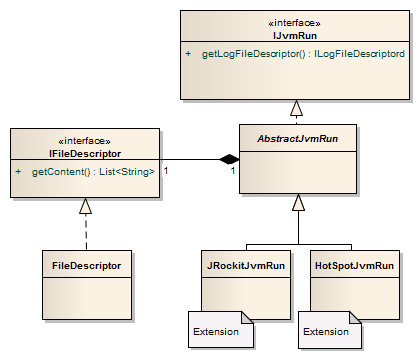
\includegraphics[width=16cm]{images/core_domain}
\end{figure}
\textit{IFileDescriptor} wird für die Abstraktion der Garbage Collection Log Datei verwendet. Darin enthalten sind Metadaten wie Dateiname und Pfad sowie der Inhalt der Datei - dieser wird allerdings erst beim öffnen der Analyse geladen (lazy). Das Basis-Modell beinhaltet zusätzlich eine naive Abstraktion eines Runs: \textit{IJvmRun} und \textit{AbstractJvmRun}. Diese werden dann in der jeweiligen Extension realisiert (Beispiel: \textit{JRockitJvmRun}). 

\subsection{Profil (Benutzerdefinierte Auswertung) erstellen}
Die Definition von benutzerdefinierten Charts kann innerhalb von Profilen gespeichert werden. Diese Profile werden in einer Übersicht dargestellt und sind gruppiert nach der jeweiligen Extension (Beispiel: JRockit). Sofern eine Log-Datei geöffnet oder selektiert ist, kann durch Doppelklick auf ein gespeichertes Profil die Analyse dafür geöffnet werden. Die Implementation der View-Domäne befindet sich in der jeweiligen Extension. Damit das Profil über die View ``Profiles'' ersichtlich ist, muss es \textit{IProfile} realisieren.
\subsubsection{Domänenmodell}
 \begin{figure}[H]
  	\centering
        	\caption{Domänenmodell: Profilverwaltung}
    	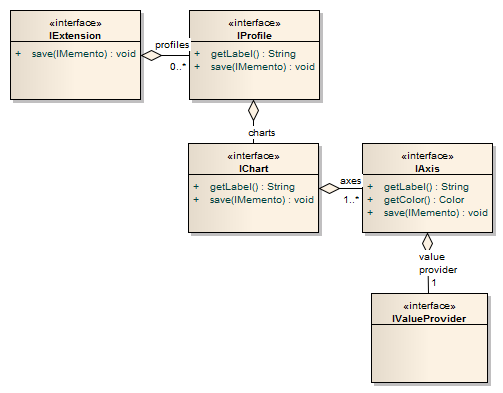
\includegraphics[width=13cm]{images/core_domain_profiles}
\end{figure}
\textit{IConfiguration} die zur Gruppierung der Profile. Pro Extension wird eine Konfiguration mit einer unbestimmten Anzahl an Profilen gespeichert. Innerhalb eines Profils können unterschiedliche Diagramme (\textit{IChart}) angelegt werden, welche wiederum durch Achsen (\textit{IAxis}) und deren Daten. Die Abfrage der Daten findet über sogenannte \textit{IValueProvider} statt. Diese definieren den Weg, wie die Daten aus dem Domänen-Modell gelesen werden.

\subsubsection{Charts definieren}
\subsubsection{Profil speichern}
Die erstellten Profile mit den darin definierten Charts müssen über die Grenze der Session hinweg gespeichert werden. Ein dafür mögliches Design Pattern wurde durch die Gang of Four\footnote{Erich Gamma, Richard Helm, Ralph Johnson, John Vlissides} in \cite[S. 283]{gamma1995design} definiert. Mit dem Prinzip des Mementos (siehe \titleref{memento}) wird garantiert, dass sie auch über die Zeit einer Session gespeichert bleiben. Für die Speicherung der Profile wird beginnend vom Root-Objekt (\textit{IExtension}), auf der Basis des Visitor-Patterns\cite[S. 331]{gamma1995design}, ein Memento-Objekt erstellt. Dieses wird anschliessend im Eclipse-Context (dieser überlebt Shutdown und Restart der Workbench) oder als XML auf dem Datei-System gespeichert. 

\subsubsection{Profil exportieren}
\subsubsection{Profil importieren}
\subsubsection{Hilfesystem}
Das Hilfesystem der Eclipse Entwicklungsumgebung ist als Client-Server-Lösung implementiert. Beim Start der Entwicklungsumgebung wird zusätzlich ein Jetty-Server gestartet, der die Hilfeseiten und Dienste wie die Suche und Indizierung bereitstellt. Die Hilfeseiten werden in zwei unterschiedliche Arten unterteilt:
\begin{itemize}
\item \textbf{Indexbasierte Hilfen:} Für die generellen Informationen und Hilfen werden verschiedene Hilfeseiten basierend auf einem Index bereitgestellt. Die Inhalte sind nicht an ein Fenster oder eine Aktion des Benutzers gebunden. 
\item \textbf{Kontextsensitive Hilfen:} Tipps die im Zusammenhang mit einer Aktion oder eines Fensters eines Benutzers stehen werden mit den Kontextsensitiven Hilfen implementiert. Bei diesen Hilfen besteht eine Verbindung zwischen Fenstern, Aktionen auf der einen Seite und den Hilfeseiten auf der Anderen.
\end{itemize}



\section{JRockit Erweiterung}
\subsection{Garbage Collection Log Datei parsen}
Die Garbage Collection Logs der JRockit Virtual Machine bestehen aus Einträgen unterschiedlicher Log Module. Genauer genommen können die Ausgaben betreffend Garbage Collection und Memory Allokation per Kommandozeile eingeschaltet werden (siehe Abschnit \ref{logmodule} \titleref{logmodule}). Für die Garbage Collection Analyse sind nur ein Teil dieser Einträge interessant - es werden also niemals alle dieser Einträge von der Analyse-Software verstanden. Für die Analyse der Einträge ist der \textit{JRockitAnalyzer} zuständig.Die Einträge werden durch einen Prozessor, der nach dem Chain-of-Responsibility Pattern\cite{wiki:chainOfResponsibilityPattern} aufgebaut ist, prozessiert. Die wichtigsten Einträge des Garbage Collection Logs sind die des Memory Modules und werden vom 
\textit{MemoryModuleProzessor} geparst. Die gelesenen Daten werden interpretiert und innerhalb des Domänenmodells abgelegt. Das Chain-of-Responsibility Pattern ermöglicht es an dieser Stelle, neue Funktionalität in Form von neuen oder erweiterten Prozessoren zu definieren.

 \begin{figure}[H]
  	\centering
        	\caption{JRockit Analyseprozess}
    	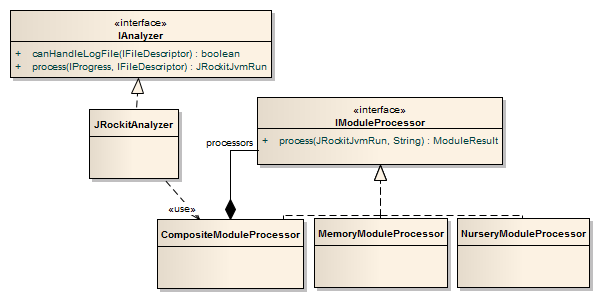
\includegraphics[width=16cm]{images/jrockit_log_processing}
\end{figure}

\subsection{Domänenmodell JRockit Garbage Collection}
\begin{landscape}
 \begin{figure}[H]
  	\centering
        	\caption{Domänenmodell: Garbage Collection (JRockit Implementation)}
    	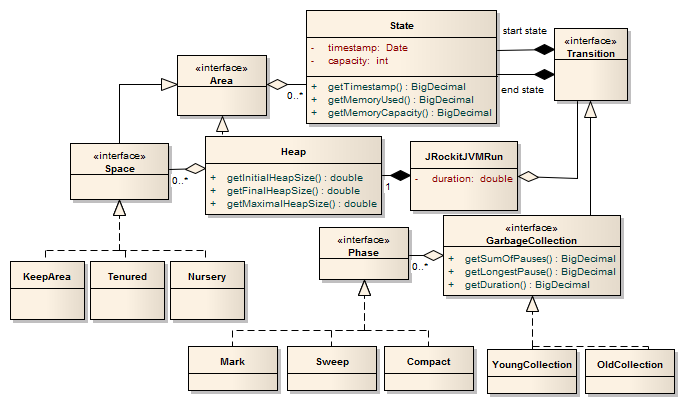
\includegraphics[width=19.5cm]{images/jrockit_extension_domain}
\end{figure}
\end{landscape}

Die Daten der Log-Datei repräsentieren einen Lauf einer JVM (\textit{JRockitJVMRun}) bestehend aus einem Heap und den darin enthaltenen Bereichen Keep-Area, Nursery und Tenured Space. Für all diese Bereiche sind unterschiedliche Zustände definiert. Obwohl sich die Zustände der einzelnen Bereiche kontinuierlich verändern, wird bei Beginn und Ende der Garbage Collection ein Schnappschuss produziert und es werden die verfügbaren Messgrössen aufgezeichnet. Zustandsübergänge werden in der Automatentheorie als Transitionen bezeichnet, werden hier im Domänenmodell aber als Garbage Collection Zyklen 
registriert. Es kann sich dabei bei der JRockit Virtual Machine um Young oder Old Collections handeln. Das starten einer Transition wird durch einen Event ausgelöst (hier im Diagramm nicht ersichtlich), Events werden aufgrund von heuristischen Daten der Lauzeitumgebung ausgelöst - zum Beispiel wenn die Nursery oder die Old Collection voll ist, etc. Der Vollständigkeit halber sind im Diagramm zusätzlich noch die einzelnen Phasen der Garbage Collection definiert. Je nach Algorithmus folgt die Sweep-Phase oder Kopaktierung auf eine Markierungs-Phase.


\subsection{Standardauswertung anzeigen}
\subsubsection{Anzeige Übersicht Garbage Collection}
Der initiale Tab der Analyseseite zeigt verschiedene zusammenfassende Daten des Garbage Collection Logs. Diese werden folgendermassen tabellarisch dargestellt:
\begin{itemize}
	\item Heap Kapazität
	\begin{itemize}
		\item Initiale Kapazität (Nursery, Tenured, Heap)
		\item Maximale Kapazität (Heap)
		\item Speicherbedarf Peak (Heap)
		\item Kapazität Durchschnittlich (Heap)
		\item Speicherbedarf Durchschnittlich (Heap)
	\end{itemize}
	\item Garbage Collection Aktivität (Young und Old Collection)
	\begin{itemize}
		\item Letzter Zyklus
		\item Anzahl Zyklen
		\item Durchschnittlicher Interval in Sekunden
		\item Durchschnittliche Dauer in Sekunden		
	\end{itemize}	
	\item Gesamtstatistik
	\begin{itemize}
		\item Dauer der Messung in Sekunden
		\item Anzahl Garbage Collection Zyklen
		\item Total Zeit der Garbage Collection
		\item Prozentuale Zeit der Garbage Collection
		\item Totale Zeit der Old Garbage Collection Zyklen
		\item Prozentuale Zeit der Old Garbage Collection Zyklen
	\end{itemize}
\end{itemize}

\subsubsection{Chart Anzeige Heap Benutzung}
Die Heap-Analyse zeichnet den Verlauf des benutzten Speichers im Heap über die Zeit auf. Die einzelnen Garbage Collection Zyklen inklusive der Farbe als Kennzeichnung Young, Old Collection werden als Punkte im Chart markiert.

\subsubsection{Chart Anzeige Dauer Garbage Collection}
Die Dauer der einzelnen Garbage Collection Zyklen wird gegenüber der verstrichenen Laufzeit dargestellt. Die einzelnen Garbage Collection Zyklen inklusive der Farbe als Kennzeichnung Young, Old Collection werden werden als Punkte im Chart markiert.


%--------------------------------------------
\section{Lizenzierung}
Die Software wird lizenziert unter der Eclipse Public License\footnote{http://www.eclipse.org/legal/epl-v10.html} in der Version 1.0. Dies ist eine freie Software-Lizenz und gewährt das Recht zur freien Nutzung, Weiterverbreitung und Veränderung der Software. Die Benutzung einer Open-Source Lizenz hat insbesondere folgende Vorteile:
\begin{itemize}
	\item An der Entwicklung von Open-Source Software können sich eine beliebige Anzahl an Entwicklern beteiligen. Der Entwicklungsaufwand kann skaliert werden.
	\item Jedermann kann Erweiterungen entwickeln oder Fehler beheben.
\end{itemize}

Bei der Wahl der Lizenz muss gleichzeitig in Betracht gezogen werden, dass die Lizenzen der verwendeten Bibliotheken ebenfalls eingehalten werden. Übersicht der verwendeten Bibliotheken:

\begin{longtable}{|p{3cm}|p{7cm}|p{4cm}|}
    \caption{Verwendete Bibliotheken und deren Lizenzen}\\\hline
	\textbf{Bibliothek} & \textbf{Beschreibung}  & \textbf{Lizenz}\\\hline
	Eclipse Framework & Framework zur Erstellung von Destkop-Anwendungen. & Eclipse Public License\\\hline 
	JFreeChart & Wird für im Bereich des Reportings verwendet um Graphiken und Charts anzuzeigen. & Lesser General Public License\footnote{http://www.gnu.org/licenses/lgpl.html}\\\hline
\end{longtable}



\section{Internationalisierung (I18n)}
Basierend auf dem Lokalisierungssystem der Java Virtual Machine kann man in Eclipse alle Spracheressourcen in Properties-Dateien auslagern (Eclipse bietet dafür sogar einen Wizard). Normalerweise liefert man die Default-Sprache innerhalb des Projektes für welches die Ressource-Bundles definiert wurden, erweiterte Sprachpackete werden dann als Fragmente ausgeliefert. Den Sprachwechsel der Eclipse Entwicklungsumgebung muss man allerdings in der Eclipse-Konfigurationsdatei eclipse.ini vollziehen - dieser benötigt auch immer einen Neustart der Entwicklungsumgebunt.

\section{Testing}\label{testing}
In Nicht-Plugin-Projekten legt man den Test-Code in einem zusätzlichen Quelltext-Ordner an (Beispielsweise src/main/java und src/main/test). Damit ist der Zugriff auf package-private\footnote{Felder und Methoden ohne Deklaration der Sichtbarkeit (private, protected, public) sind in Java implizit package-private - sie sind also für alle Subklassen und innerhalb des selben Ordners (Package) sichtbar. } Felder und Methoden ebenfalls möglicht, zusätzlich bleibt der Test-Code von der Implementation getrennt. Dieses vorgehen wird auch vom Build-Werkzeug Maven Tycho unterstützt. Wenn man das entsprechende Test-Plugin als Eclipse-Test-Plugin konfiguriert\footnote{Dies kann innerhalb der Maven-Konfigurationsdatei pom.xml mit dem Element packaging gemacht werden.}, können die Tests auch während dem Build automatisiert durchgeführt werden.

Bei Eclipse-Plugin-Projekten erstellt man für den Test-Code ein separates Projekt. In das zu verteilende Softwarepacket (Feature) werden nur die Nicht-Test-Plugins getan. Der Zugriff vom Test-Projekt auf die Implementationen ist per se nicht möglich\footnote{Jedes Plugin muss definieren, welche Packages für die anderen Plugins sichtbar sind.}, zu diesem Zweck wird das Test-Projekt als Fragment definiert.

%--------------------------------------------
\section{Infrastruktur}
\subsection{Build-Automation}
Die Automatisierung des Software-Builds ist hinsichtlich der Integration in ein Continuous Integration System Voraussetzung. Es hat zusätzlich aber andere Vorteile:
\begin{itemize}
	\item Tasks wie das Kompilieren, die Packetierung und das Deployment der Software müssen nicht mehr manuell gemacht werden.
	\item Zur Verhinderung von Regression und entsprechend zur Gewährleistung der Qualität können vor jedem Release automatisch die Tests durchgeführt werden.
\end{itemize}

Als Werkzeug zum automatisierten Build der Software wird Maven Tycho\footnote{Im Bereich der Eclipse Rich Client Entwicklung kann entweder PDE Build, ein auf Apache Ant basiertes Build-System für Eclipse RCP Applikationen\cite{vogelZapfPdeBuild} oder die Maven-Integration Tycho (http://tycho.sonatype.org) verwendet werden.} verwendet. Um Tycho führt mittlerweile kein Weg drum herum, es hat im Vergleich zum PDE Build einige Vorteile:
\begin{itemize}
	\item Maven Builds lassen sich ohne grossen Aufwand in Continuous Integration Systeme integrieren.
	\item Maven hat eine gute Integration in alle gängigen Entwicklungsumgebungen\footnote{Projekt-Dateien müssen nicht mehr in die Versionskontrolle eingecheckt werden.} und ist sehr verbreitet
\end{itemize}

\subsection{Continous Integration}
Als Continuous Integration Server wird Jenkins\footnote{http://jenkins-ci.org - Jenkins ist der ehemalige Hudson CI Server, welcher nach dem Kauf von Sun durch Oracle als Branch entstanden ist.} verwendet. Jenkins bringt nebst seiner Benutzerfreundlichkeit als Build Server einige zum Projekt nötigen Voraussetzungen mit:
\begin{itemize}
	\item Jenkins ist für alle denkbaren Betriebssysteme vorhanden.
	\item Jenkins ist kompatibel mit allen gängigen Systemen zur Versionskontrolle: Git, Subversion, CVS, etc.
	\item Maven-Projekte lassen sich ohne grossen Aufwand als Build-Projekte konfigurieren.
\end{itemize}

\subsection{Versionskontrolle}
Zur Versionskontrolle kommen mehrere Werkzeuge in Frage. Git\footnote{http://git-scm.com} ist ein verteiltes Sourcecode Management System und ist konzeptionell und hinsichtlich Benutzerfreundlichkeit besser als Subversion und CVS\footnote{Git kann offline verwendet werden, das Verschieben von Verzeichnissen führt nicht zu Problemen, etc.}. Auf der Plattform Github\footnote{http://github.com} kann man öffentliche Projekte gratis ``hosten''.

\subsection{Issue Tracker}
Als Issue Tracker wird Jira verwendet. Es handelt sich dabei um eine kostenpflichtige aber relativ günstige Software für das Issue-Tracking.

\subsection{Installation der Software}\label{installation}
Zur Installation der Software benötigt man die Eclipse-Entwicklungsumgebung in der Version 3.7. Darin integriert befindet sich ein Update-Manager, der Software-Komponenten von Lokal oder dem Netzwerk installieren kann. Auch Updates werden über diesen Mechanismus installiert. Die Analyse-Software wird via eine Update-Seite bereitgestellt. Der Software-Build durch das Continuous Integration System publiziert die Artefakte (Features, Plugins) auf einen via Internet zugänglichen Rechner, von welchem der Update-Manager die Software herunterlädt um anschliessend zu importieren. Update-Seiten im Eclipse-Umfeld bestehen aus Features (Eclipse Feature-Projekt). Features bestehen aus unterschiedlichen Plugins (Eclipse Plugin-Projekt). Eclipse\footnote{in der Basis ist es Equinox, die Implementation des OSGi Standards} ist in der Lage, Plugins zur Laufzeit zu installieren, starten, deinstallieren.

Die Update-Seite für diese Software wird folgendermassen aufgebaut:
\begin{itemize}
	\item Garbage Collection Log Analysis (Kategorie)
		\begin{itemize}
			\item Core (Feature)
			\item JRockit Extension (Feature)
		\end{itemize}
\end{itemize}
Nachträglich kann somit auch für ein anderes Log-Format eine Extension geschrieben werden.


